\documentclass[a4paper]{article}
\usepackage[T1]{fontenc}
\usepackage[utf8]{inputenc}
\usepackage{fancyhdr}
\usepackage{hyperref}
\usepackage{tikz}
\usepackage{listings}
\usepackage{caption}
\usetikzlibrary{decorations.pathmorphing,shapes,arrows,positioning,calc,fit,petri}
\setlength\parindent{0pt}
%% == Commands ================================================
\newcommand{\coursecode}{TDA297}
\newcommand{\coursename}{Distributed Systems II (Advanced)}
\newcommand{\authorname}{Sebastian Weddmark Olsson, Erica Löfström}
\newcommand{\authormail}{sebastiw@student.chalmers.se, lofstrom.erica@gmail.com}
\newcommand{\doctitle}{Tentalösningar}
\newcommand{\horrule}[1]{\rule{\linewidth}{#1}} % Create horizontal rule command with 1 argument of height
\newcommand{\oklarhet}[1]{%
  \noindent\fbox{\parbox[b][4em][t]{\textwidth}{\color{red}#1} }%
}
\newcommand{\points}[1]{\subsection{} \textit{#1 points}\\}
\newcommand{\question}[2][]{
  \noindent
  \parbox[t]{\textwidth}{#1 \parbox[t]{0.95\textwidth}{#2}}\\
}
\newcommand{\seealso}[1]{\\\textit{See also:} #1}
\newcommand{\solution}[1]{\\\horrule{0.5pt}\\[3pt]\textit{Solution: }\\[0.1cm]\begin{minipage}{\textwidth}#1\end{minipage}}
\newcommand{\highlight}[1]{{\color{blue}#1}}


%% == Settings ================================================
\setlength{\topskip}{0pt} % Skip some whitespace at the top
\pagestyle{fancy}
\topmargin -20.0pt
\headheight 56.0pt
\rhead{
  \coursename\\
  \doctitle
}

\tikzset{
  bend angle     = 15,
  pre/.style     = {<-,shorten <=1pt, semithick},
  post/.style    = {->,shorten >=1pt, semithick},
  process/.style = {draw, circle, node distance=3cm},
  doorway/.style={draw, rectangle, minimum height=2cm, text width=2cm},
  group/.style={draw, rectangle, dashed},
  skip loop/.style={to path={-- ++(0,#1) -| (\tikztotarget)}}
}

\newsavebox{\userinput}

%% == Document ================================================
\begin{document}


\thispagestyle{plain} % No header for first page
\begin{center}
\horrule{0.5pt} \\[0.3cm] % Thin top horizontal rule
%
\huge \coursecode -- \coursename \\[1mm]
\Large \doctitle \\
\normalsize % Revert to normal sized font
\horrule{2pt} \\[0.1cm] % Thick bottom horizontal rule
\begin{tabular}{ l r }
Av \authorname & \authormail
\end{tabular}\\[0.1cm]
\footnotesize \today\\[0.4cm]
\end{center}
{\footnotesize
Please feel free to spread the document to anyone that wants it, and please improve the solutions if you can. All of the document, as well as the \LaTeX{} code, is public domain.
Note! These solutions are not from the department giving the course, and they have not been checked for errors. The answers might not be explicit enough to give full points.\\
}
\horrule{0.5pt} % Thin top horizontal rule
\normalsize % Revert to normal sized font
\\[2.5cm]

%% == Solutions ================================================
\section{Tenta 2012-03-05}

\points{10}
\question{
  Give an example of an execution that is sequential consistent but
  not linearizable. \\
  Show that every linearizable history is sequential consistent.
}
\seealso{\ref{2014-03:linearizability}, \ref{2013-08:linearizability}, \ref{2013-03:linearizability}}
\solution{See: \ref{2013-03:linearizability}}

\points{10}
\question{
  Give a specification of a state machine replication abstraction and
  an underlying algorithm to implement it using a total order broadcast
  abstraction.
}
\oklarhet{Bad formulation of the question?}
\solution{
  An replica manager (RM) can be a state machine, which has the
  following properties:\\
  State Machine
  \begin{itemize}
    \item Applies operations atomically.
    \item Its state is a deterministic function of its internal state
      and the operations applied.
    \item All replicas start identical and carry out the same sequence
      of operations.
    \item Its operations must not be affected by clock readings etc.
  \end{itemize}

  ISIS algorithm for total ordering broadcast:\\
  Each process $p$ keeps $A^q$, the largest agreed sequence number it
  has observed so far, and $P^q$, its own largest proposed sequence
  number.
  \begin{enumerate}
    \item $p$ B-multicasts <$m$,$i$> where $i$ is a unique identifier
      for message $m$.
    \item On receiving <$m$,$i$> for the first time
      Each process $q$ replies to the sender $p$ with a proposal
      for the message's agreed sequence number of $P^q := Max(A^q,
      P^q)+1$. Each process provisionally assigns the proposed
      sequence number to the message and places it in its hold-back
      queue. Which is ordered with the smallest sequence number at the front.
    \item $p$ collects all proposed sequence numbers and selects the
      largest one, $a$, as the next agreed sequence number. It then
      B-multicasts <$i$,$a$>. Each process $q$ sets $A^q := Max(A^q,
      a)$, and attaches $a$ to the message (which is identified by
      $i$). If the agrees sequence number differs from the proposed
      sequence number, it reorders the messages in its hold-back
      queue. When the message at the front of the hold-back queue has
      been assigned its agreed sequence number, it is transferred to
      the tail of the delivery queue. Messages that have been assigned
      their agreed sequence number but are not at the head of the
      hold-back queue, are not yet transferred.
  \end{enumerate}

  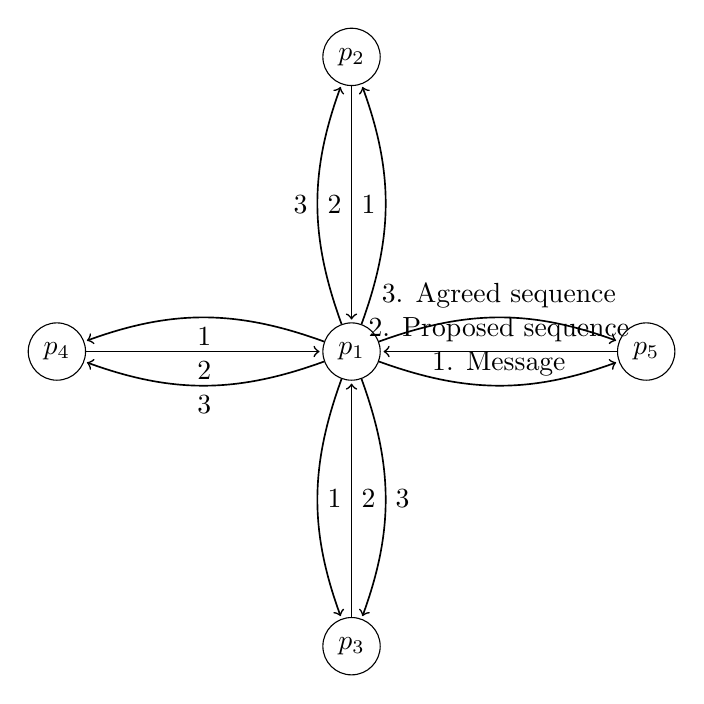
\begin{tikzpicture}[bend angle=20]
    \node[process] (p1)               {$p_1$};
    \node[process] (p2) [above=of p1] {$p_2$}
    edge [pre, bend right] node[auto, swap] {3} (p1)
    edge [pre, bend left]  node[auto, swap] {1} (p1)
    edge [post]            node[auto, swap] {2} (p1);
    \node[process] (p3) [below=of p1] {$p_3$}
    edge [pre, bend right] node[auto, swap] {3} (p1)
    edge [pre, bend left]  node[auto, swap] {1} (p1)
    edge [post]            node[auto, swap] {2} (p1);
    \node[process] (p4) [left=of p1]  {$p_4$}
    edge [pre, bend right] node[auto, swap] {3} (p1)
    edge [pre, bend left]  node[auto, swap] {1} (p1)
    edge [post]            node[auto, swap] {2} (p1);
    \node[process] (p5) [right=of p1] {$p_5$}
    edge [pre, bend right] node[auto, swap] {3. Agreed sequence}  (p1)
    edge [pre, bend left]  node[auto, swap] {1. Message} (p1)
    edge [post]            node[auto, swap] {2. Proposed sequence} (p1);
  \end{tikzpicture}
}


\points{5}
\question{
  Is it possible to implement a total order broadcast
  deterministically in asynchronous systems with message loses? \\
  Provide an algorithm or an impossibility proof.
}
\solution{
  No, it is not possible. Proof equivalent to the consensus problem.\\
  Consensus problem:\\
  To reach consensus every process $p_i$ begins in the undecided
  state and proposes a single value $v_i$, drawn from a set $D$ ($i =
  1, 2, ..., N$). The processes communicate with one another,
  exchanging values. Each process then sets the value of a decision
  variable, $d_i$. In doing so it enters the decided state, in which
  it may no longer change $d_i$ ($i = 1, 2, ..., N$). \\

  The requirements of a consensus algorithm are that the following
  conditions should hold for every execution of it:
  \begin{description}
    \item[Termination] every correct process eventually decides some
      value.
    \item[Validity] if all processes that propose a value proposes $v$
      then all correct processes eventually decide $v$.
    \item[Agreement] if a correct process decides on value $v$, then all correct
      processes eventually decides on $v$.
    \item[Integrity] every process decides at most once, and if it
      decides some value $v$ then $v$ must have been proposed by some process.
  \end{description}

  %% Maybe tikz?
  % \begin{tikzpicture}
  % \end{tikzpicture}
}

\points{10}
\label{2012-03:causal}
\question{
  What are the properties that a causal broadcast must satisfy? \\
  Compare the causal broadcast property with the following property:
  ``if a process delivers messages $m_1$ and $m_2$, and $m_1 \rightarrow
  m_2$, then the process must deliver $m_1$ before $m_2$.''
}
\oklarhet{Unsure about the comparison in the question and answer.}
\solution{
  Causality properties:
  \begin{description}
    \item[FIFO order] Some process $p_i$ broadcasts $m_1$ before
      broadcasting $m_2$.
    \item[Local order] Some process $p_i$ delivers $m_1$ and then
      broadcasts $m_2$.
    \item[Transitivity] There is a message $m'$ such that $m_1
      \rightarrow m'$ and $m' \rightarrow m_2$.
  \end{description}

  In order for the causal broadcast property (``if a process delivers
  messages $m_1$ and $m_2$, and $m_1 \rightarrow m_2$, then the
  process must deliver $m_1$ before $m_2$.'') to happen, either a
  process must have broadcasted $m_1$ and $m_2$ in order, or a process
  have delivered $m_1$ and then broadcasts $m_2$ as a response to
  $m_1$, or there is some message $m'$ that happened before $m_2$ but
  not before $m_1$ such that $m_1 \rightarrow m', m' \rightarrow m_2$.
}

\points{10}
\question{
  The flooding algorithm is a straight forward broadcasting
  algorithm. The initiator sends to all its neighbors a message of kind
  broadcast. When a process receives message broadcast for the first
  time, it sends to all other adjacent processes further broadcast
  messages. \\
  What is the Time and Message Complexity of the algorithm? Please
  provide a complexity analysis.
}
\solution{
  In a graph $G(V,E)$ where $V$ is the processes, the number of
  messages needed is $2|E|$, and the time complexity is the depth
  (diameter) of the graph $D(G)$.

  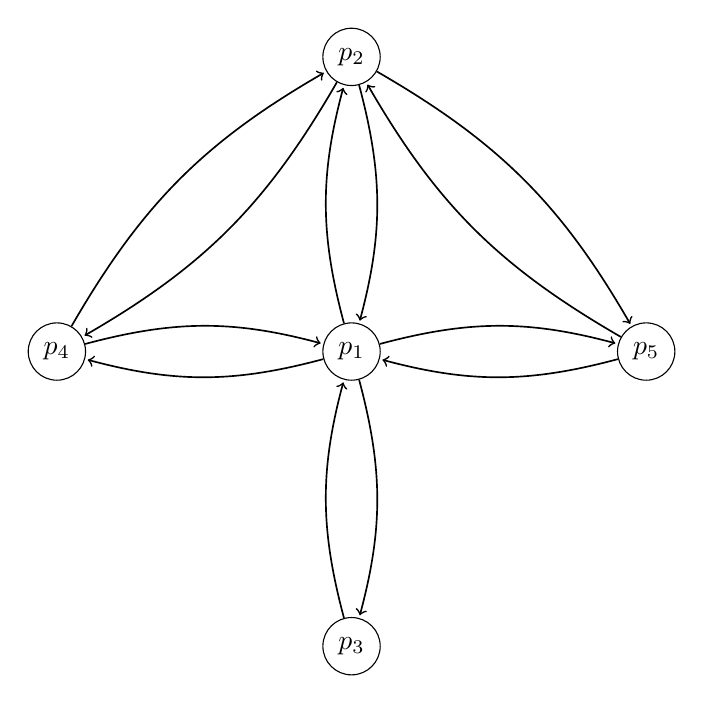
\begin{tikzpicture}
    \node[process] (p1)               {$p_1$};
    \node[process] (p2) [above=of p1] {$p_2$}
    edge [pre, bend right] (p1)
    edge [post, bend left] (p1);
    \node[process] (p3) [below=of p1] {$p_3$}
    edge [pre, bend right] (p1)
    edge [post, bend left] (p1);
    \node[process] (p4) [left=of p1]  {$p_4$}
    edge [pre, bend right] (p1)
    edge [post, bend left] (p1)
    edge [pre, bend right] (p2)
    edge [post, bend left] (p2);
    \node[process] (p5) [right=of p1] {$p_5$}
    edge [pre, bend right] (p1)
    edge [post, bend left] (p1)
    edge [pre, bend right] (p2)
    edge [post, bend left] (p2);
  \end{tikzpicture}

  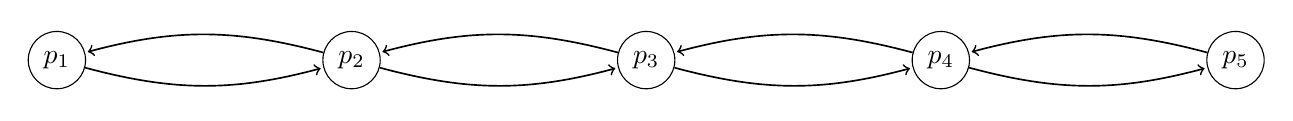
\begin{tikzpicture}
    \node[process] (p1)               {$p_1$};
    \node[process] (p2) [right=of p1] {$p_2$}
    edge [pre, bend left] (p1)
    edge [post, bend right] (p1);
    \node[process] (p3) [right=of p2] {$p_3$}
    edge [pre, bend left] (p2)
    edge [post, bend right] (p2);
    \node[process] (p4) [right=of p3] {$p_4$}
    edge [pre, bend left] (p3)
    edge [post, bend right] (p3);
    \node[process] (p5) [right=of p4] {$p_5$}
    edge [pre, bend left] (p4)
    edge [post, bend right] (p4);
  \end{tikzpicture}
}

\points{10}
\question{
  The algorithm by Choy and Singh uses two Doorways. The Asynchronous
  and the Synchronous Doorway. \\ Describe them in pseudo-code and
  informally. \\ Use both Doorways to construct a solution to the
  Dinning Philosophers problem for a system of 3 philosophers.
}
\solution{
  Let $N_p$ denote the set of neighbors of process $p$ and $L_{pq}$
  the actual state of $q$ known by $p$. If neighbor processes
  $q_0,...,q_t \in N_p$ have entered the doorway, $p$ must wait until
  $q_0,...,q_t$ will have exited the doorway.\\[0.1cm]

  Asynchronous Doorway entry code:\\
  $\forall q \in N_p:$ \textbf{wait until} $L_{pq} \neq m_1$;\\
  \textbf{broadcast} message $m_1$ to all neighbors;\\[0.1cm]

  Asynchronous Doorway exit code:\\
  \textbf{broadcast} a message different from $m_1$ to neighbors;\\[0.1cm]

  Synchronous Doorway entry code:\\
  \textbf{wait until} ($\forall q \in N_p: L_{pq} \neq m_2$);\\
  \textbf{broadcast} message $m_2$ to neighbors;\\[0.1cm]

  Synchronous Doorway exit code:\\
  \textbf{broadcast} a message different from $m_2$ to neighbors;\\[0.1cm]

  The problem the asynchronous doorway is that $n$ processes can all
  enter the doorway at the same time, because it takes some time to
  actually enter the doorway.\\[0.1cm]

  The problem with the synchronous doorway is that two processes can
  cooperate to block a third process. It is not fair.\\[0.1cm]

  To solve the Dinning philosophers problem, a double doorway is
  needed.\\
  The entry code consists out of the synchronous doorway entry code
  embedded in an asynchronous doorway entry and exit code. Processes
  that wish to enter the double doorway cannot forever be hindered from
  entering by neighbour processes as the asynchronous doorway will allow
  a process to proceed latest when all neighbors inside the doorway
  have passed the asynchronous doorway exit code. Further the
  asynchronous doorway guarantees that process $p$ which passed the
  asynchronous doorway will be blocked from entering the synchronous
  doorway at most once by each neighbor.

  %% Master thesis p.50.
  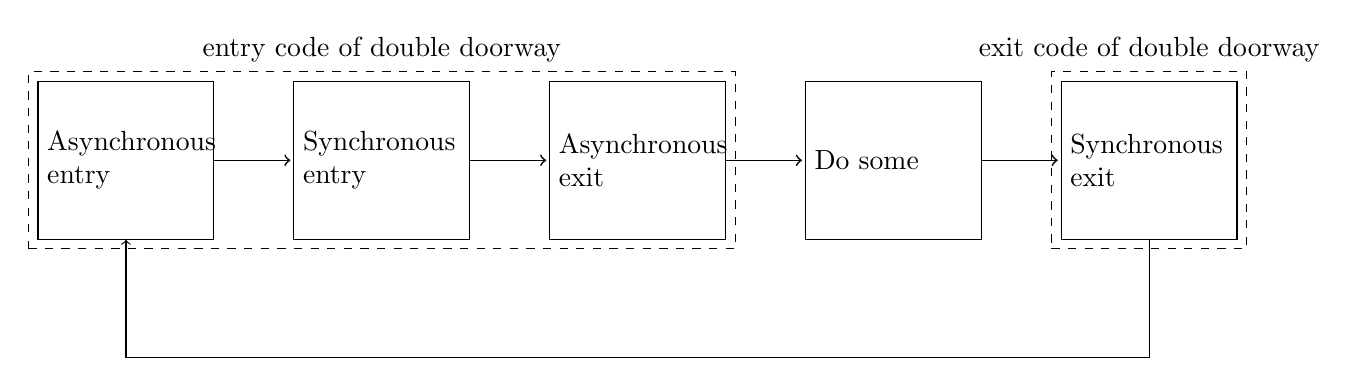
\begin{tikzpicture}
    \node[doorway] (async entry) [] {Asynchronous entry};
    \node[doorway] (sync entry)  [right=of async entry] {Synchronous entry}
    edge [pre] (async entry);
    \node[doorway] (async exit)  [right=of sync entry] {Asynchronous exit}
    edge [pre] (sync entry);
    \node[doorway] (dosome)  [right=of async exit] {Do some}
    edge [pre] (async exit);
    \node[doorway] (sync exit)  [right=of dosome] {Synchronous exit}
    edge [pre] (dosome)
    edge [->,skip loop=-25mm] (async entry);


    \begin{scope}
      \node [group, fit=(async entry) (sync entry) (async exit), label=above:{entry code of double doorway}]
      (entry box) {};
    \end{scope}

    \begin{scope}
      \node [group, fit=(sync exit), label=above:{exit code of double doorway}]
      {};
    \end{scope}
  \end{tikzpicture}
}

\points{5}
\label{2012-03:byzantine}
\question{
  Show that Byzantine agreement can be reached for three generals, if
  the generals digitally sign their messages.
}
\solution{
  The Byzantine generals problem differs from consensus in that a distinguished
  process supplies a value that the others are to agree upon, instead of each of them
  proposing a value. The system needs to be synchronous because a crashed process is
  indistinguishable from a slow one in an asynchronous system.\\

  The number of faulty processes $f$ allowed to still reach consensus when messages are not
  digitally signed is $ f < N/3 $, where $N$ is the total number of processes.

  \begin{minipage}{0.45\linewidth}
    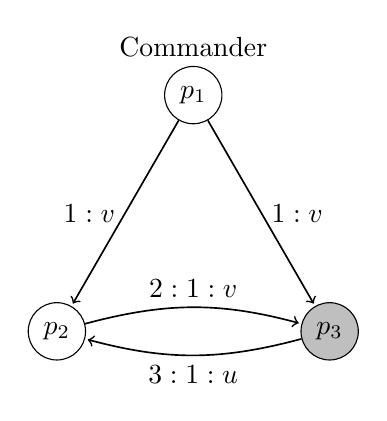
\begin{tikzpicture}
      \node[process] (g1) at (90:2) [label=above:{Commander}] {$p_1$};
      \node[process] (g2) at (210:2) {$p_2$}
      edge [pre] node [left] {$1:v$} (g1);
      \node[process, fill=black!25] (g3) at (330:2) {$p_3$}
      edge [pre] node [right] {$1:v$} (g1)
      edge [pre, bend right] node [above] {$2:1:v$} (g2)
      edge [post, bend left] node [below] {$3:1:u$} (g2);
    \end{tikzpicture}
  \end{minipage}
  \begin{minipage}{0.45\linewidth}
    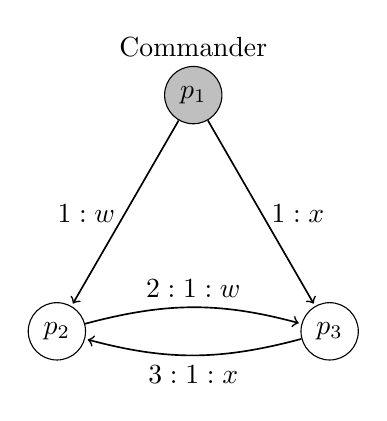
\begin{tikzpicture}
      \node[process, fill=black!25] (g1) at (90:2) [label=above:{Commander}] {$p_1$};
      \node[process] (g2) at (210:2) {$p_2$}
      edge [pre] node [left] {$1:w$} (g1);
      \node[process] (g3) at (330:2) {$p_3$}
      edge [pre] node [right] {$1:x$} (g1)
      edge [pre, bend right] node [above] {$2:1:w$} (g2)
      edge [post, bend left] node [below] {$3:1:x$} (g2);
    \end{tikzpicture}
  \end{minipage}

  In the picture above, messsage $2:1:v$ can be read as $p_2$ says that $p_1$
  ordered $v$. In the left picture, $p_2$ gets one order from $p_1$
  and a different order from $p_3$; there is no telling who is
  faulty. The right picture, where the commander is faulty, the same
  conclusion can be drawn. In neither cases, $p_2$ cannot distinguish
  which process that is faulty.

  The solution to this problem is to digitally sign messages.

  The assumption is that every message carries a signatue, and the
  signature cannot be forged, hence alteration of the contents of a
  sign message can be detected. Every non-faulty process can verify
  the signature of any other non-faulty process.

  Any number $f$ of faulty processes is allowed.

  \begin{minipage}{0.45\linewidth}
    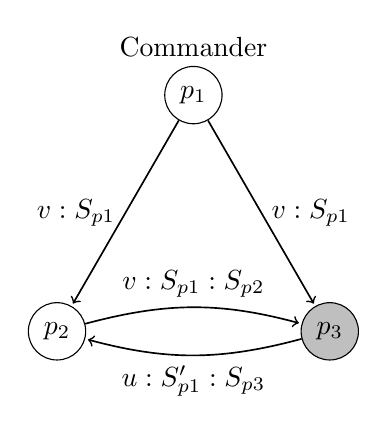
\begin{tikzpicture}
      \node[process] (g1) at (90:2) [label=above:{Commander}] {$p_1$};
      \node[process] (g2) at (210:2) {$p_2$}
      edge [pre] node [left] {$v:S_{p1}$} (g1);
      \node[process, fill=black!25] (g3) at (330:2) {$p_3$}
      edge [pre] node [right] {$v:S_{p1}$} (g1)
      edge [pre, bend right] node [above] {$v:S_{p1}:S_{p2}$} (g2)
      edge [post, bend left] node [below] {$u:S'_{p1}:S_{p3}$} (g2);
    \end{tikzpicture}
  \end{minipage}
  \begin{minipage}{0.45\linewidth}
    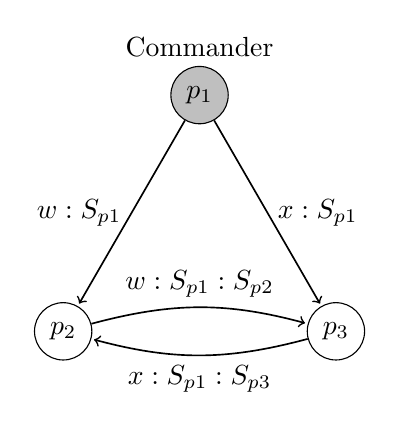
\begin{tikzpicture}
      \node[process, fill=black!25] (g1) at (90:2) [label=above:{Commander}] {$p_1$};
      \node[process] (g2) at (210:2) {$p_2$}
      edge [pre] node [left] {$w:S_{p1}$} (g1);
      \node[process] (g3) at (330:2) {$p_3$}
      edge [pre] node [right] {$x:S_{p1}$} (g1)
      edge [pre, bend right] node [above] {$w:S_{p1}:S_{p2}$} (g2)
      edge [post, bend left] node [below] {$x:S_{p1}:S_{p3}$} (g2);
    \end{tikzpicture}
  \end{minipage}

  In the pictures above, $x:S_{p1}:S_{p2}$ is the value x, signed by
  both $p_1$ and $p_2$. In the left picture, process $p_2$ discovers
  that $p_1$s signature has been tampered with; $p_3$ is the traitor.
  In the right picture, both processes $p_2, p_3$ get non-tampered
  messages, with different values; $p_1$ is the traitor.
}

\section{2012-08}
\points{10}
\question{
  Construct a solution to reliable, totally ordered multicast
  in a synchronous system, using a reliable multicast and a solution
  to the consensus problem.
}
\solution{
  R-multicast(g, m)
    uniquely tag m with sender and sequence number
    send(m) to all processes in group g (including self)
  end

  R-deliver(m)
  upon receive(g, m) where process p in g do
  if p have not already delivered m
  then if p is not sender of m
  then send m to all neighbors in g
  endif
  deliver(m)
  endif
  end
}

\points{5}
\question[a)]{
  Can Byzantine agreement be reached for 8 generals, with 3 of them
  faulty?
}
\question[b)]{
  Can Byzantine agreement be reached for 8 generals, with 3 of them
  faulty, if the generals digitally sign their messages?
}
\solution{
  see \ref{2012-03:byzantine}
}

\points{8}
\question{
  A three-phase commit protocol has the following parts \\
  \textbf{Phase 1:} is the same as the two phase commit.\\
  \textbf{Phase 2:} the coordinator collects the votes and makes a
  decision; if it is No, it aborts and informs participants hat voted
  Yes, if the decision is Yes, it sends a precommit request to all
  participants. Participants that voted Yes wait for a precommit or
  doAbort request. They acknowledge precommit requests and carry out
  doAbort requests. \\
  \textbf{Phase 3:} the coordinator collects the acknowledgements When
  all are received, it commits and sends a do commit to the
  participants. Participants wait for a doCommit request. When it
  arrives they Commit. \\
  Explain how this protocol avoids delay to participants during their
  ``uncertain'' period due to the failure of the coordinator or other
  participants. Assume that communication does not fail.
}
\solution{
  If the state of the cohorts is before precommit and no
  precommit-message is sent from the coordinator, then each cohort
  assumes a failure and abort the commit. If the cohorts have received
  a precommit-message, but does not get a commit-message from the
  coordinator, then they will automatically commit.
}

\points{10}
\question{
  A processor P is part of a network G(V,E). P believes that processor
  Q is also connected to the network. Describe a protocol that P
  together with the other processors of the network can use in order to
  find Q or to find that Q is not part of the network. Prove the time
  complexity of the algorithm.
}
%
\begin{lrbox}{\userinput}
  \begin{minipage}{\linewidth}
    \begin{lstlisting}[mathescape]
      init_echo () {
        N = {q | q is a neighbor of p}
        for each q in N
        send token to q
        counter = 0
        while( counter < |N| ) {
          receive token
          counter++
        }
        terminate
      }

      echo() {
        receive token from parent
        N = {q | q is neighbor of p != parent}
        for each q in N
        send token to q
        counter = 0
        while( counter < |N| ) {
          receive token
          counter++
        }
        send token to parent
        terminate
      }
    \end{lstlisting}
  \end{minipage}
\end{lrbox}
%
\solution{
  Our assumption is that an initiator $P$ wants to find out if a
  process $Q$ exists in G(V,E).


  Broadcasting with ACK = Echo algorithm\\
  Creates a spanning tree.

  \usebox{\userinput}

  This algorithm can be used, if we change the answer to the parent to
  either ``i have Q in my section of the graph'' or ``i dont know
  where Q is''.
  When the initiator $P$ have collected all answers, then he knows if
  $Q$ is part of the network or not.

  Phase 1 (when all nodes have been reached) takes $O(D)$ time, where
  $D$ is the depth of the graph. In Phase 2, the distance between the 
  initiator and processes having received all acknowledgements have been 
  decreased by at least 1. So it takes $O(n)$ time for this phase to complete.
  Because $ n >= d $, it takes $O(n)$ time to complete the whole
  algorithm.
}

\points{15}
\question{
  Give a solution to the dinning philosophers problem. Prove the time
  complexity of the algorithm.
}\\
%
\begin{lrbox}{\userinput}
  \begin{minipage}{\linewidth}
    Let $G(V,E)$ be a communication graph of the modeled network, for which $V$ denotes the set
    of processes and $E$ the set of links between processes of $V$. Then, every process $p \in V$
    represents a philosopher, who works independently and may request resources at any time. Further
    for every resource which is shared between two processes $p$ and $q$ there exist a link $(p,q) \in E$
    and vice versa. Thus, every process can request directly resources from its neighbors. A resource
    is represented by a token called \textit{fork}.\\
    It is assumed that every process can be in one of the following states: \textit{thinking, hungry} 
    or \textit{eating}. A process in state \textit{thinking} is not interesed in its neighbors resources
    and sends requested forks to its neighbors. A process will switch from \textit{thinking, hungry} when
    it wants to access its resource. Then it tries to collect all forks from its neighbors. When a process
    in state \textit{hungry} collects all forks from its neighbors it will start accessing its resources. 
    It changes to state \textit{eating} in which it keeps all forks until it finishes with accessing the
    resources and changes to thinking again. 
    \begin{enumerate}
	\item The algorithm is initialized by an acyclic precedence graph H and all processes
	with lower precedence own dirty forks while processes with higher precedence own
	request tokens. All processes are initially thinking, i.e. they are not interested
	in their resources. 
	\item A process which becomes hungry will send all its request token to neighbor 
	processes and wait until it received all forks. 
	\item A process which received all forks will change its state to \textit{eating}
	\item A process which leaves the critical section (stops eating) changes the state 
	of all its forks to \textit{dirty}. Then for all held request token the respective
	fork is sent to neighbor processes.	
    \end{enumerate}
    The above steps assume the following: 
    \begin{itemize}
	\item \textit{Receiving a request token for fork f}: If processors state is different
	than \textit{eating} and $f$ is dirty then $f$ will be sent to the requesting processor.
	If processors state was also \textit{hungry} then the request token will also be sent back.
	\item \textit{Receiving a fork f}: The state of $f$ will be set to clean. 
    \end{itemize}
  \end{minipage}
\end{lrbox}
%
\solution{
  See \ref{2014-03:doorways} for solution with doorways.\\ 
  In dining philosophers problem five or more philosophers (processes) dines
  together at a table. The philosophers has three states: \textit{thinking, hungry} and \textit{eating}.
  Between each of the two philosophers lies one fork, i.e. the philosophers shares forks between eachother.
  In order for a philosopher to eat he must aquire both his left and his right fork. The main problem is to
  guarantee no deadlock, where no one can eat because no one has two forks, and no starvation, where one
  hungry philosopher never gets to eat.\\
  To solve this problem, the Chandy and Misra algorithm can be used, as described below:\\\\
  \usebox{\userinput}
  Time complexity:
  A process at depth $k$ will have to wait for forks from neighbors with lower precedence time $2(d+l)$
  plus the time from neighbors of depth $k-1$ needs to be able to eat.

From the correctness proof it can be concluded that a process at depth k will have
to wait for forks from neighbours with lower precedence time 2( d + l ) plus the time
neighbours of depth k 1 needs to be able to eat. This results in following recursion:
;
T ( k ) = T ( k ; 1) + 4( d + l )
4( k + 1)( d + l )
Although the acyclic graph is initially of depth , the worst case depth is
transformations of H . Therefore, a process must wait time O ( n ( d + l )) .

}


\points{12}
\question{
  A quorum consensus method with three replicas is used for
  replication. The parameters of the replication system are described in
  the following table. Calculate: \textit{i)} the read latency,
  \textit{ii)} the write latency, \textit{iii)} the blocking probability
  of a read and \textit{iv)} the blocking probability of a write.}

\oklarhet{Unsolvable since a part of the question is missing.}

\section{Tenta 2014-03-12}
\points{10}
\label{2014-03:linearizability}
\question[a)]{
  Give the definitions of Linearizability and Sequential Consistency.
}
\question[b)]{
  A correctness property $\rho$ is compositional if, whenever
  each object in the system satisfies $\rho$, the system as a whole
  satisfies $\rho$. Is Sequential Consistency compositional? \\
  If yes explain why, if no give an example.
}
\solution{
a) A replicated shared object service is said to be \highlight{linearzable} if there is some interleaving in the series of operations issued by all clients that satisfies the following criterias:
\begin{itemize}
  \item{The interleaving sequence of operations meets the specifications of a (single) correct copy of the objects}
  \item{\highlight{The order of operations in the interleaving is consistent with the real times at which the operations occured in the actual execution}}
\end{itemize}
A replicated shared object service is said to be \highlight{sequentially consistent} is there is some interleaving in the series of operations issued by all clients that satisfies the following criterias:
\begin{itemize}
  \item{The interleaving sequence of operations meets the specifications of a (single) correct copy of the objects}
  \item{\highlight{The order of operations in the interleaving is consistent with the program order at which individual client executed them}}
\end{itemize}
b) Sequential consistency is not compositional. If sequential consistency were compositional then the combination of separate sequential concistent implementations of two objects yields a sequential consistent implementation. This doesn't hold in the following example:
  \begin{center}
    \begin{tabular}{| l | l |}\hline
      Client 1: & Client 2: \\\hline
      $setBalance_B(x, 1)$ &\\
      & $getBalance_A(y) \rightarrow 0$\\
      & $getBalance_A(x) \rightarrow 0$\\
      $setBalance_A(y, 2)$ &\\\hline
    \end{tabular}
  \end{center}
   When there are two objects the execution is sequentially consistent. But if these two clients executed on just one object, as below the execution is no longer sequentially consistent. In the example below client 1 sets the balance of the object to 1 and Client 2 reads the balance as 0 and therefore the execution is not sequentially consistent. Hence, sequential consistency is not compositional. 
  \begin{center}
    \begin{tabular}{| l | l |}\hline
      Client 1: & Client 2: \\\hline
      $setBalance_A(x, 1)$ &\\
      & $getBalance_A(y) \rightarrow 0$\\
      & $getBalance_A(x) \rightarrow 0$\\
      $setBalance_A(y, 2)$ &\\\hline
    \end{tabular}
  \end{center}
}

\points{10}
\label{2014-03:phase-commit}
\question{
  Describe the differences between the three-phase commit
  protocol and the two-phase commit protocol. Draw the three-phase
  commit protocol as a state machine where you also describe the
  behavior of the protocol when time-outs are triggered and processes
  are recovered after crashing.}
%
\begin{lrbox}{\userinput}
  \begin{minipage}{0.5\linewidth}
    \captionsetup{width=0.75\textwidth} 
    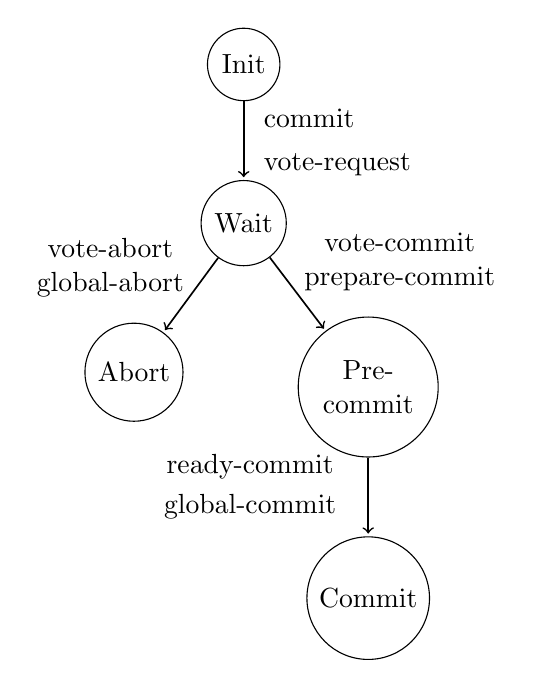
\begin{tikzpicture}[node distance=1cm]
      \node[process] (init) [] {Init};
      \node[process] (wait) [below=1cm of init] {Wait}
      edge [pre]
      node [label=15:{commit}, label=-15:{vote-request}] {}
      (init);
      \node[process] (abort) [below left=1.5cm of wait, xshift=0.5cm] {Abort}
      edge [pre]
      node[] {} 
      (wait);
      \node[process] (precommit) [below right=1.5cm of wait, xshift=-0.5cm, align=center,text width=1.3cm] {Pre\-commit}
      edge [pre]
      node [] {}
      (wait);
      \node[process] (commit) [below=1cm of precommit] {Commit}
      edge [pre]
      node [] {}
      (precommit);
      %Labels
      \node [above=0.7cm of abort, xshift=-0.3cm] {vote-abort};
      \node [above=0.2cm of abort, xshift=-0.3cm] {global-abort};
      \node [above=0.7cm of precommit, xshift=0.4cm] {vote-commit};
      \node [above=0.2cm of precommit, xshift=0.4cm] {prepare-commit};
      \node [above=0.6cm of commit, xshift=-1.5cm] {ready-commit};
      \node [above=0.1cm of commit, xshift=-1.5cm] {global-commit};
    \end{tikzpicture}
    \captionof{figure}{The finite state \mbox{machine} for the coordinator}
  \end{minipage}
  
  \begin{minipage}{0.5\linewidth}
    \centering
    \captionsetup{width=0.75\textwidth} 
    \begin{tikzpicture}[node distance=1cm]
      \node[process] (init) [] {Init};
      \node[process] (ready) [below=1cm of init] {Ready}
      edge [pre]
      node [label=15:{vote-request}, label=-15:{ready-commit}] {}
      (init);
      \node[process] (abort) [below left=1.5cm of ready, xshift=0.5cm] {Abort}
      edge [pre]
      node [] {}
      (ready)
      edge [pre, bend left=50]
      node [] {}
      (init);
      \node[process] (precommit) [below right=1.5cm of wait, xshift=-0.5cm, align=center, text width=1.3cm] {Pre\-commit}
      edge [pre]
      node [] {}
      (ready);
      \node[process] (commit) [below=1cm of precommit] {Commit}
      edge [pre]
      node [] {}
      (precommit);
      %Labels
      \node [above=2.7cm of abort, xshift=-1cm] {vote-request};
      \node [above=2.2cm of abort, xshift=-1cm] {vote-abort};
      \node [above=0.55cm of precommit, xshift=0.4cm] {prepare-commit};
      \node [above=0.05cm of precommit, xshift=0.4cm] {ready-commit};
      \node [above=0.4cm of commit, xshift=1.3cm] {global-commit};
      \node [above=0cm of commit, xshift=1.3cm] {ACK};
    \end{tikzpicture}
    \captionof{figure}{The finite state \mbox{machine} for a participant}
  \end{minipage}
\end{lrbox}
%
\solution{
  The difference between the two-phase commit protocol (2PC)
  and the three-phase commit protocol (3PC) is that in 3PC all
  participants enter a pre-commitment state before commiting.
  The 2PC protocol has the limitation that it is a blocking 
  protocol. For example, if the coordinator crashes while 
  receiveing replies from the can commit query so that some reply
  are lost, the coordinator restarts and believes that some processes
  has not yet decided and blocks indefinitely waiting for the lost
  replies. Participants can also be stuck in an indefinitely block
  if messages from the coordinator is lost.
  The 3PC protocol is not a blocking protocol so it does not have 
  those issues. Also, due to timeouts the processes is not stuck in 
  a state indefinitely.
\usebox{\userinput}
  Coordinator:\\
  If the coordinator crashes before sending a vote request to the 
  participants the coordinator aborts upon restart. Otherwise the
  coordinator sends a vote request to the participants and move
  on to the waiting phase.\\
  If there is a failure, timeout or if the coordinator receives a
  voting abort message the coordinator sends out a global abort to
  the participants and aborts. Otherwise, if all vote commit messages
  is received before the timeout, the coordinator sends out a prepare
  commit message to the participants and move to the precommit phase. 
  If the coordinator crashes during the prepare commit messages sending
  the coordinator can just continue with the sending of prepare commit
  messages after reboot.\\ 
  If the coordinator receives ready commit from all participants a global
  commit message is sent out to the participants and the coordinator
  commits. Otherwise, if there is a failure or timeout the coordinator
  aborts. \\\\
  %
  Participant:\\ 
  If a participant crashes after receiving a vote request, the 
  participant aborts and replies with vote abort to the coordinator.
  The participant also votes abort if it cannot commit even though 
  no crash has occured. Otherwise it replies with a vote commit message
  and moves to the ready phase. \\
  If in the prepared state, the participant recieves an abort message
  from the coordinator, it fails or it times out waiting for a message
  the participant aborts. If the participant receives a prepare commit
  message it replies with an ACK and moves to the precommit phase. \\
  If coordinator crashes after the participants has received prepare 
  commit messages the participants goes forward with the commit. 
}
%
%
\points{5}
\question{
  What are the properties that a causal broadcast must satisfy? \\
  Compare the causal broadcast property with the following property:
  ``if a process delivers messages $m_1$ and $m_2$, and $m_1 \rightarrow
  m_2$, then the process must deliver $m_1$ before $m_2$.''
}
\solution{See:~\ref{2012-03:causal}}
%
\points{10}
\question[a)]{
  Describe an algorithm for leader election on a ring topology. All
  processes have unique ids and the system is asynchronous. Any process
  can initiate the leader election protocol at any time.
}
\question[b)]{
Compute the time complexity and communication complexity of
  your algorithm.
}
\question[c)]{
  Is it possible to design a symmetric algorithm for leader
  election? If yes, provide such an algorithm, if no provide a proof.
}
%
\solution{
a) The assumption is that no failure occurs and that the processes are
  connected in a ring topology. \\
  Initially all processes are marked as non-participant and their leader
  variable is set to $\bot$ (unidentified). The initiating process marks
  itself as participant and sends an election message containing its 
  own process identifier to its clockwise neighbour. \\
  When receiving an election message, the process compare its own id with
  the id in the message. If the id of the process is smaller than the id
  in the message, the process marks itself as participant and forwards the
  message to its neighbour. If the process id is greater than the id in the
  message and the process is marked as non-participant, then the process
  marks itself as participant, changes the id in the election message to 
  its own id and forwards the message. However if the process already was 
  marked participant the process don't do anything. If the identifier in 
  the message is the same as the process own id the process becomes the 
  elected leader. The process sets its own id in its leader variable, marks
  itself as non-participant and then sends out an elected message containing
  its own id. When a process recieves the elected message it marks itself
  as non-participating and sets the leader varible to the identifier in 
  the message. Then it forwards the elected message to its neighbour if its
  neighbour isn't the elected leader. \\ \\
  
  It's immediate from the correctness proof that the protocols terminates after exactly N+1 rounds.

To count message traffic, observe that each process sends at most 1 message per round, for a total of O(N2) messages. This is a tight bound since if the ids are in decreasing order N N-1 N-2 ... 1, then no messages get eaten until they hit N. 
  
  b) Time complexity: 
  In worst case the processes are ordered in ascending order and the process
  with the lowest process id initiates the election. Since the messages only
  can travel one node at a time the election message must travers through the 
  ring twice in the worst case. The elected message always traverses through the 
  ring once and the total nr of messges in the protcol becomes $3n-1$ messages.
  Hence the time complexity is $O(n)$. \\
  %
  Communcation complexity:
  If all processes starts election at the same time the multiple election messages
  will be discarded once a participating process with a higher id than the one in
  the message receives it. A message can be discarded in $1$ up to $N$ steps. 
  Therefore, the communcation complexity is $O(n^2)$
}
%
\points{15}
\question[a)]{
  Eric wants to build a replicated storage system. In his
  system there is only one client. The client performs just one
  storage operation (read or write) at a time, waiting for each
  operation to complete before starting the next. Eric wants
  availability even in the case of one server failure. Because of that
  he decides to store the data on two servers. Eric wants to ensure
  that the data on the two servers stay identical all the time. In
  order to guarantee that he is thinking making the two servers atomic
  using three-phase commit, to ensure both-or-nothing behavior. In the
  design he has in mind, the client acts as the transaction
  coordinator. The client would execute a write as described in the
  three-phase commit protocol. The system uses timeout recovery scheme
  explaineed in the lectures. Eric thinks about this design for a
  while, and eventually realizes that three-phase commit is
  fundamentally not suited to providing availability via
  replication. \\
  Please explain why. Eric wants to formalize the consistency
  properties of the replication system. Is it sequential consistent?
  Is it a linearizable one? Please explain your answer.
}
\question[b)]{
  Eric decides to change his design and uses now the gossip
  architecture that lazily synchronizes the two servers. The single
  client contacts any server that is available and gets the value that
  this server has, updates are also performed on the first available
  server first and then lazily propagated on the next server. Each
  client request uses a unique id.\\
  What is the availability that he can achieve? Eric wants to
  formalize the consistency properties of the replication system in
  case where there are no failures. Is it sequential consistent? Is it
  a linearizable one? Please explain your answer.
}
\question[c)]{
  Eric decides to change his design and uses now nine replicas
  and quorums to ensure strong consistency and availability. What are
  the constraints on the sizes of read and write quorums? What is the
  availability that he can achieve? Give an example of quorum
  processing involving a write, two reads, then a write. Eric wants
  to formalize the consistency properties of the replication
  system. Is it sequential consistent? Is it a linearizable one?
  Please explain why?
}

\points{10}
\label{2014-03:doorways}
\question{
  The algorithm by Choy and Singh uses two Doorways. The
  Asynchronous and the Synchronous Doorway. \\
  Describe them in pseudo-code and informally. \\
  If we use the Asynchronous Doorway together with coloring, is this
  algorithm going to give us a solution to the resource allocation
  problem (e.g. is it going to guarantee mutual exclusion and
  no-starvation)? Please provide a proof sketch or a
  counterexample. \\
  What is the time complexity of this algorithm?
}

\section{Tenta 2013-03-16}
\points{10}
\label{2013-03:linearizability}
\question[a)]{
  Give the definitions of Linearizability and Sequential Consistency
}
\question[b)]{
  Give an example pseudocode for a simple program that
  would operate correctly with sequential consistency but incorrectly
  with linearizability. (Briefly explain your answer.)
}
\question[c)]{
  Describe the advantages and disadvantages of using each
  for an application, paying particular attention to any assumptions
  you must make about the users behaviour. As two example applications
  you can consider:
  \begin{itemize}
    \item a web site allowing registered users to upload videos and
      allowing anybody to download and watch them. (Comments on videos
      are note supported.)
    \item a multi-user game, the players move figures around a common
      scene. The state of the game is replicated at the players'
      workstation and a server. The figures may throw projectiles at
      another, and a hit debilitates the unfortunate recipient for a
      limited time. (Application II is from Chapter 18th of the course
      book.)
  \end{itemize}
}
\solution{
  A replicated shared object service is said to be
  \highlight{linearizable} if \textit{for any execution} there is
  some interleaving of the series of operations issued by all the
  clients that satisfies the following two criteria:
  \begin{itemize}
    \item The interleaved sequence of operations meets the
      specification of a (single) correct copy of the objects.
    \item The order of operations in the interleaving is consistent
      with the \highlight{real times at which the operations
        occurred in the actual execution.}
  \end{itemize}

  A replicated shared object service is said to be
  \highlight{sequentially consistent} \textit{if for any
    execution} there is some interleaving of the series of operations
  issued by all the clients that satisfies the following two criteria:
  \begin{itemize}
    \item The interleaved sequence of operations meets the
      specification of a (single) correct copy of the objects.
    \item The order of operations in the interleaving is consistent
      with the \highlight{program order in which each individual
        client executed them.}
  \end{itemize}

  \begin{center}
    Example execution for a service which is sequentially consistent
    but not linearizable.\\
    \begin{tabular}{| l | l |}\hline
      Client 1: & Client 2: \\\hline
      $setBalance_B(x, 1)$ &\\
      & $getBalance_A(y) \rightarrow 0$\\
      & $getBalance_A(x) \rightarrow 0$\\
      $setBalance_A(y, 2)$ &\\\hline
    \end{tabular}
    The real-time criterion for linearizability is not satisfied,
    since $getBalance_A(x) \rightarrow 0$ occurs later than
    $setBalance_B(x,1)$.\\
  \end{center}

  Sequential consistency requires that all of the data
  \textit{appears} to have been executed atomically, in some sequential
  order that is consistent with the order seen at the individual
  processes. When this order must also preserve the global (external)
  ordering of non-overlapping operations, this consistency guarantee is
  called linearizability.
}


\points{10}
\question[a)]{What are FIFO ordering, causal ordering and total
  ordering guarantees of replica managers? How are they related to
  each other?}
\question[b)]{Compare the causal ordering property with the following
property: ``if a replica manager processes messages $m_1$ and $m_2$,
and $m_1 \rightarrow m_2$, then the replica manager must process $m_1$
before $m_2$.''}

\points{10}
\question[a)]{Eric wants to build a replicated storage system. In his
  system there is only one client. The client performs just one
  storage operation (read or write) at a time, waiting for each
  operation to complete before starting the next. Eric wants
  availability even in the case of one server failure. Because of that
  he decides to store the data on two servers. Eric wants to ensure
  that the data on the two servers stay identical all the time. In
  order to guarantee that he is thinking making the two servers atomic
  using two-phase commit, to ensure both-or-nothing behavior. In the
  design he has in mind, the client acts as the transaction
  coordinator. The client would execute a write as described in the
  two-phase commit protocol. The system uses timeout recovery scheme
  explaineed in the lectures. Eric thinks about this design for a
  while, and eventually realizes that two-phase commit is
  fundamentally not suited to providing availability via
  replication. \\
  Please explain why.}
\question[b)]{Eric decides to change his design and use nine replicas
  and quorums to ensure strong consistency and availability. What are
  the constraints on the sizes of read and write quorums? What is the
  availability that he can achieve? Give an example of quorum
  processing involving a write, two reads, then a write.}


\points{10}
\question{A distributed conference application provides a shared
  whiteboard. Each member of the conference has a replica of the
  whiteboard that is managed by a specific member of a closed process
  group. \\
  Describe an approach that uses the algorithm by Choy and Singh to
  achieve mutually exclusive access to the whiteboard, prior to
  propagation of the updates to the whole group. \\
  If the number of members of the group is $n$, what is the time
  complexity of the scheme, provide a brief proof?}

\points{5}
\question{Describe an algorithm that solves consensus in a synchronous
  system where up to $f$ of the $n$ processes exhibit crash failures,
  assume the existence of a reliable multicast protocol. \\
  What is the time complexity of the algorithm.}

\points{10}
\question{The flooding algorithm is a straight forward reliable
  broadcast algorithm. The initiator sends to all its neigbors a
  message of kind broadcast. When a process receives message broadcast
  for the first time, it sends to all other adjacent processes
  further broadcast messages.}
\question[a)]{What are the properties of reliable broadcast.}
\question[b)]{What is the Time and Message Complexity of the algorithm
  in fault-free asynchronous execution?}
\question[c)]{What is the Time and Message Complexity of the algorithm
  in an asynchronous execution in the presence of crash faults? (No
  partitions.) \\
  Please provide brief complexity analysis.}

\points{5}
\question{Consider it as given that there is no Byzantine agreement
  protocol for a system with 3 processes, from which 1 of them
  faulty. Using this proof prove that there is no Byzantine agreement
  protocol for a system with $n \geq 3$ processes, from which $f$ are
  faulty if $n \leq 3f$.}


\section{2013-08-23}
\points{10}
\question{Describe an implementation of a distributed
  Linked-List that tolerates 2 replica crashes for all operations
  (\textit{insert, delete} and \textit{find}). Your implementation
  should take care and clean unnecessary memory periodically.}

\points{10}
\label{2013-08:linearizability}
\question{Explain the difference between linearizability
  and sequential consistency.}

\points{15}
\question{Describe an algorithm that computes a spanning
  tree of a network $G(V,E)$. Explain how a node of the network can use
  the existence of such a spanning tree in order to broadcast
  information to all nodes of the network.}

\points{15}
\question{Describe the two generals problem. Can you find
  a solution to the problem? If yes describe your solution and provide a
  proof of its time and communication complexity. If not provide a proof
  that the problem is not solvable. }
% Nämn både synchronous och asynchronous system!

\points{10}
\question{Gifford's quorum consensus replication is in use
  at servers $X, Y$, and $Z$ which all hold replica's of data items $A$
  and $B$. The initial values of all replicas of $A$ and $B$ are 100 and
  the votes for $A$ an $B$ are 1 at each $X, Y$ and $Z$. Also $R=W=2$
  for both $A$ and $B$. A client reads the value of $A$ then writes it
  to $B$.}\\
\question[a]{At the time the client performs these
  operations, a particion separates server $X$ and $Y$ from server
  $Z$. Describe the quota obtained and the operations that take place if
  the client can access server $X$ and $Y$.}
\question[b]{Describe the quora obtained and the operations that take
  place if the client can access only server $Z$.}
\question[c]{The partition is repaired and then another partition
  occurs so that $X$ and $Z$ are separated from $Y$. Describe the
  quora obtained and the operations that take place if the client can
  access server $X$ and $Z$.}
\end{document}
